% Options for packages loaded elsewhere
\PassOptionsToPackage{unicode}{hyperref}
\PassOptionsToPackage{hyphens}{url}
\documentclass[
  ignorenonframetext,
]{beamer}
\newif\ifbibliography
\usepackage{pgfpages}
\setbeamertemplate{caption}[numbered]
\setbeamertemplate{caption label separator}{: }
\setbeamercolor{caption name}{fg=normal text.fg}
\beamertemplatenavigationsymbolsempty
% remove section numbering
\setbeamertemplate{part page}{
  \centering
  \begin{beamercolorbox}[sep=16pt,center]{part title}
    \usebeamerfont{part title}\insertpart\par
  \end{beamercolorbox}
}
\setbeamertemplate{section page}{
  \centering
  \begin{beamercolorbox}[sep=12pt,center]{section title}
    \usebeamerfont{section title}\insertsection\par
  \end{beamercolorbox}
}
\setbeamertemplate{subsection page}{
  \centering
  \begin{beamercolorbox}[sep=8pt,center]{subsection title}
    \usebeamerfont{subsection title}\insertsubsection\par
  \end{beamercolorbox}
}
% Prevent slide breaks in the middle of a paragraph
\widowpenalties 1 10000
\raggedbottom
\AtBeginPart{
  \frame{\partpage}
}
\AtBeginSection{
  \ifbibliography
  \else
    \frame{\sectionpage}
  \fi
}
\AtBeginSubsection{
  \frame{\subsectionpage}
}
\usepackage{iftex}
\ifPDFTeX
  \usepackage[T1]{fontenc}
  \usepackage[utf8]{inputenc}
  \usepackage{textcomp} % provide euro and other symbols
\else % if luatex or xetex
  \usepackage{unicode-math} % this also loads fontspec
  \defaultfontfeatures{Scale=MatchLowercase}
  \defaultfontfeatures[\rmfamily]{Ligatures=TeX,Scale=1}
\fi
\usepackage{lmodern}
\ifPDFTeX\else
  % xetex/luatex font selection
\fi
% Use upquote if available, for straight quotes in verbatim environments
\IfFileExists{upquote.sty}{\usepackage{upquote}}{}
\IfFileExists{microtype.sty}{% use microtype if available
  \usepackage[]{microtype}
  \UseMicrotypeSet[protrusion]{basicmath} % disable protrusion for tt fonts
}{}
\makeatletter
\@ifundefined{KOMAClassName}{% if non-KOMA class
  \IfFileExists{parskip.sty}{%
    \usepackage{parskip}
  }{% else
    \setlength{\parindent}{0pt}
    \setlength{\parskip}{6pt plus 2pt minus 1pt}}
}{% if KOMA class
  \KOMAoptions{parskip=half}}
\makeatother
\usepackage{graphicx}
\makeatletter
\newsavebox\pandoc@box
\newcommand*\pandocbounded[1]{% scales image to fit in text height/width
  \sbox\pandoc@box{#1}%
  \Gscale@div\@tempa{\textheight}{\dimexpr\ht\pandoc@box+\dp\pandoc@box\relax}%
  \Gscale@div\@tempb{\linewidth}{\wd\pandoc@box}%
  \ifdim\@tempb\p@<\@tempa\p@\let\@tempa\@tempb\fi% select the smaller of both
  \ifdim\@tempa\p@<\p@\scalebox{\@tempa}{\usebox\pandoc@box}%
  \else\usebox{\pandoc@box}%
  \fi%
}
% Set default figure placement to htbp
\def\fps@figure{htbp}
\makeatother
\setlength{\emergencystretch}{3em} % prevent overfull lines
\providecommand{\tightlist}{%
  \setlength{\itemsep}{0pt}\setlength{\parskip}{0pt}}
% Slide layout defaults for warning-clean scientific decks.
\usepackage{etoolbox}
\IfFileExists{xurl.sty}{\usepackage{xurl}}{}
\IfFileExists{seqsplit.sty}{\usepackage{seqsplit}}{\newcommand{\seqsplit}[1]{#1}}
\protected\def\breakseq#1{\seqsplit{#1}}
\protected\def\breaktt#1{\begingroup\ttfamily\seqsplit{#1}\endgroup}
\setlength{\emergencystretch}{6em}
\tolerance=5000
\hbadness=10000
\hfuzz=1pt
\setlength{\tabcolsep}{2pt}
\AtBeginEnvironment{longtable}{\tiny\renewcommand{\arraystretch}{0.86}\setlength{\tabcolsep}{1pt}}
\AtBeginEnvironment{tabular}{\tiny\renewcommand{\arraystretch}{0.86}\setlength{\tabcolsep}{1pt}}

% Natbib and cross-reference fallbacks — slides don't load natbib
% or cleveref, but combined-PDF manuscript prose may emit these
% commands. The fallback renders citations as a bracketed key list
% and cross-references as detokenized labels so slides don't fail on
% undefined control sequences or raw underscores. \providecommand is
% a no-op if packages load later.
\providecommand{\citep}[1]{[#1]}
\providecommand{\citet}[1]{#1}
\providecommand{\citealp}[1]{#1}
\providecommand{\citeauthor}[1]{#1}
\providecommand{\citeyear}[1]{#1}
\providecommand{\cref}[1]{\texttt{\detokenize{#1}}}
\providecommand{\Cref}[1]{\texttt{\detokenize{#1}}}

\newtheorem{proposition}{Proposition}
\newtheorem{hypothesis}{Hypothesis}
\usepackage{bookmark}
\IfFileExists{xurl.sty}{\usepackage{xurl}}{} % add URL line breaks if available
\urlstyle{same}
% fallback for those not using the hyperref driver hyperxmp:
\makeatletter
\@ifundefined{xmpquote}{\newcommand{\xmpquote}[1]{#1}}{}
\makeatother
\hypersetup{
  hidelinks,
  pdfcreator={LaTeX via pandoc}}

\author{\texorpdfstring{}{}}
\date{}

\begin{document}

\section{Temporal Coordination: Turns, Overlap, and
Persistence}\label{sec:temporal}

\begin{frame}[fragile,allowframebreaks]{Temporal Coordination: Turns,
Overlap, and Persistence}
The original PPPiP form is synchronous: both partners mark the surface
at the same time. DigiPPPiP separates synchrony from relationality.
Synchronous sessions still matter because joint action requires partners
to coordinate bodies, intentions, and timing, and because active
interaction is a strong candidate context for inter-brain synchrony in
cooperative and naturalistic tasks \breakseq{[@sebanz2006joint;
@czeszumski2020hyperscanning; @czeszumski2022cooperative]}. Emerging
work on online group interaction suggests that neural alignment can also
appear under virtual conditions when participants remain actively
engaged \breakseq{[@azhari2025online]}. Yet synchrony is not the only temporal
form that can support intimacy, play, or shared meaning.

Remote and delayed modes should not be described as if distance has been
solved. Distance changes the cost of coordination, common ground,
informal repair, and collaboration readiness \breakseq{[@olson2000distance]}.
Grounding theory adds a finer vocabulary: partners need evidence that a
mark, gesture, or prompt has been perceived and understood well enough
for the next contribution \breakseq{[@clark1991grounding]}. Recent
video-mediated collaborative-drawing work makes that requirement
concrete: proposal sequences depend on verbal, embodied, and
screen-based actions, and the person controlling the drawing tool can
become pivotal in coordinating joint decisions
\breakseq{[@oittinen2025videodrawing]}. DigiPPPiP's temporal design should
therefore measure not only whether users were online together, but how
the canvas supported acknowledgement, repair, turn completion,
tool-control transfer, and later re-entry into the same shared artifact.

Semisynchronous DigiPPPiP introduces alternation. Partners are present
in the same session but take turns or contribute in bursts. That mode
preserves mutual responsiveness while creating short prediction
intervals: each mark becomes a cue for anticipating the partner's next
action. It also makes repair visible: an undo, hesitation, or spoken
clarification can become part of the event stream rather than an
invisible failure. This is a natural bridge between the modeling lens in
\breakseq{[@sec:active\_inference]} and the formal narrative account in
\breakseq{[@sec:formalisms\_appendix]}.

Asynchronous DigiPPPiP changes the practice more radically. Partners
contribute at separate times, making the canvas a persistent relational
object. Asynchronous mental-health technologies show that clinical or
supportive exchange need not always be real-time to be meaningful
\breakseq{[@lagera2023asynchronous]}. For DigiPPPiP, absence becomes part of
the form: waiting, revisiting, and responding create a slower temporal
arc of curiosity and resolution. Digital-intimacy research is relevant
here because many strong-tie technologies rely on awareness, traces,
rituals, and low-pressure presence rather than continuous conversation
\breakseq{[@hassenzahl2012love; @vetere2005mediating]}.

The temporal primitives are overlap, order, delay, persistence, and
repair. Overlap supports co-action; order supports anticipation; delay
supports reflection; persistence supports return; repair supports trust
after confusion. These primitives are more fundamental than labels such
as live, remote, or asynchronous because the same interface can
instantiate them differently for different dyads. A study that logs only
a session label loses the very structure that may explain relational
meaning.

\breakseq{[@fig:dyadic\_task\_matrix]} translates these distinctions into a
staged study matrix. The matrix separates peer, mentor, and AI-assisted
roles from co-located, remote, turn-taking, and persistent
temporal-spatial conditions. It is a protocol-planning figure, not a
claim that any one condition is universally superior.

\begin{figure}
\centering
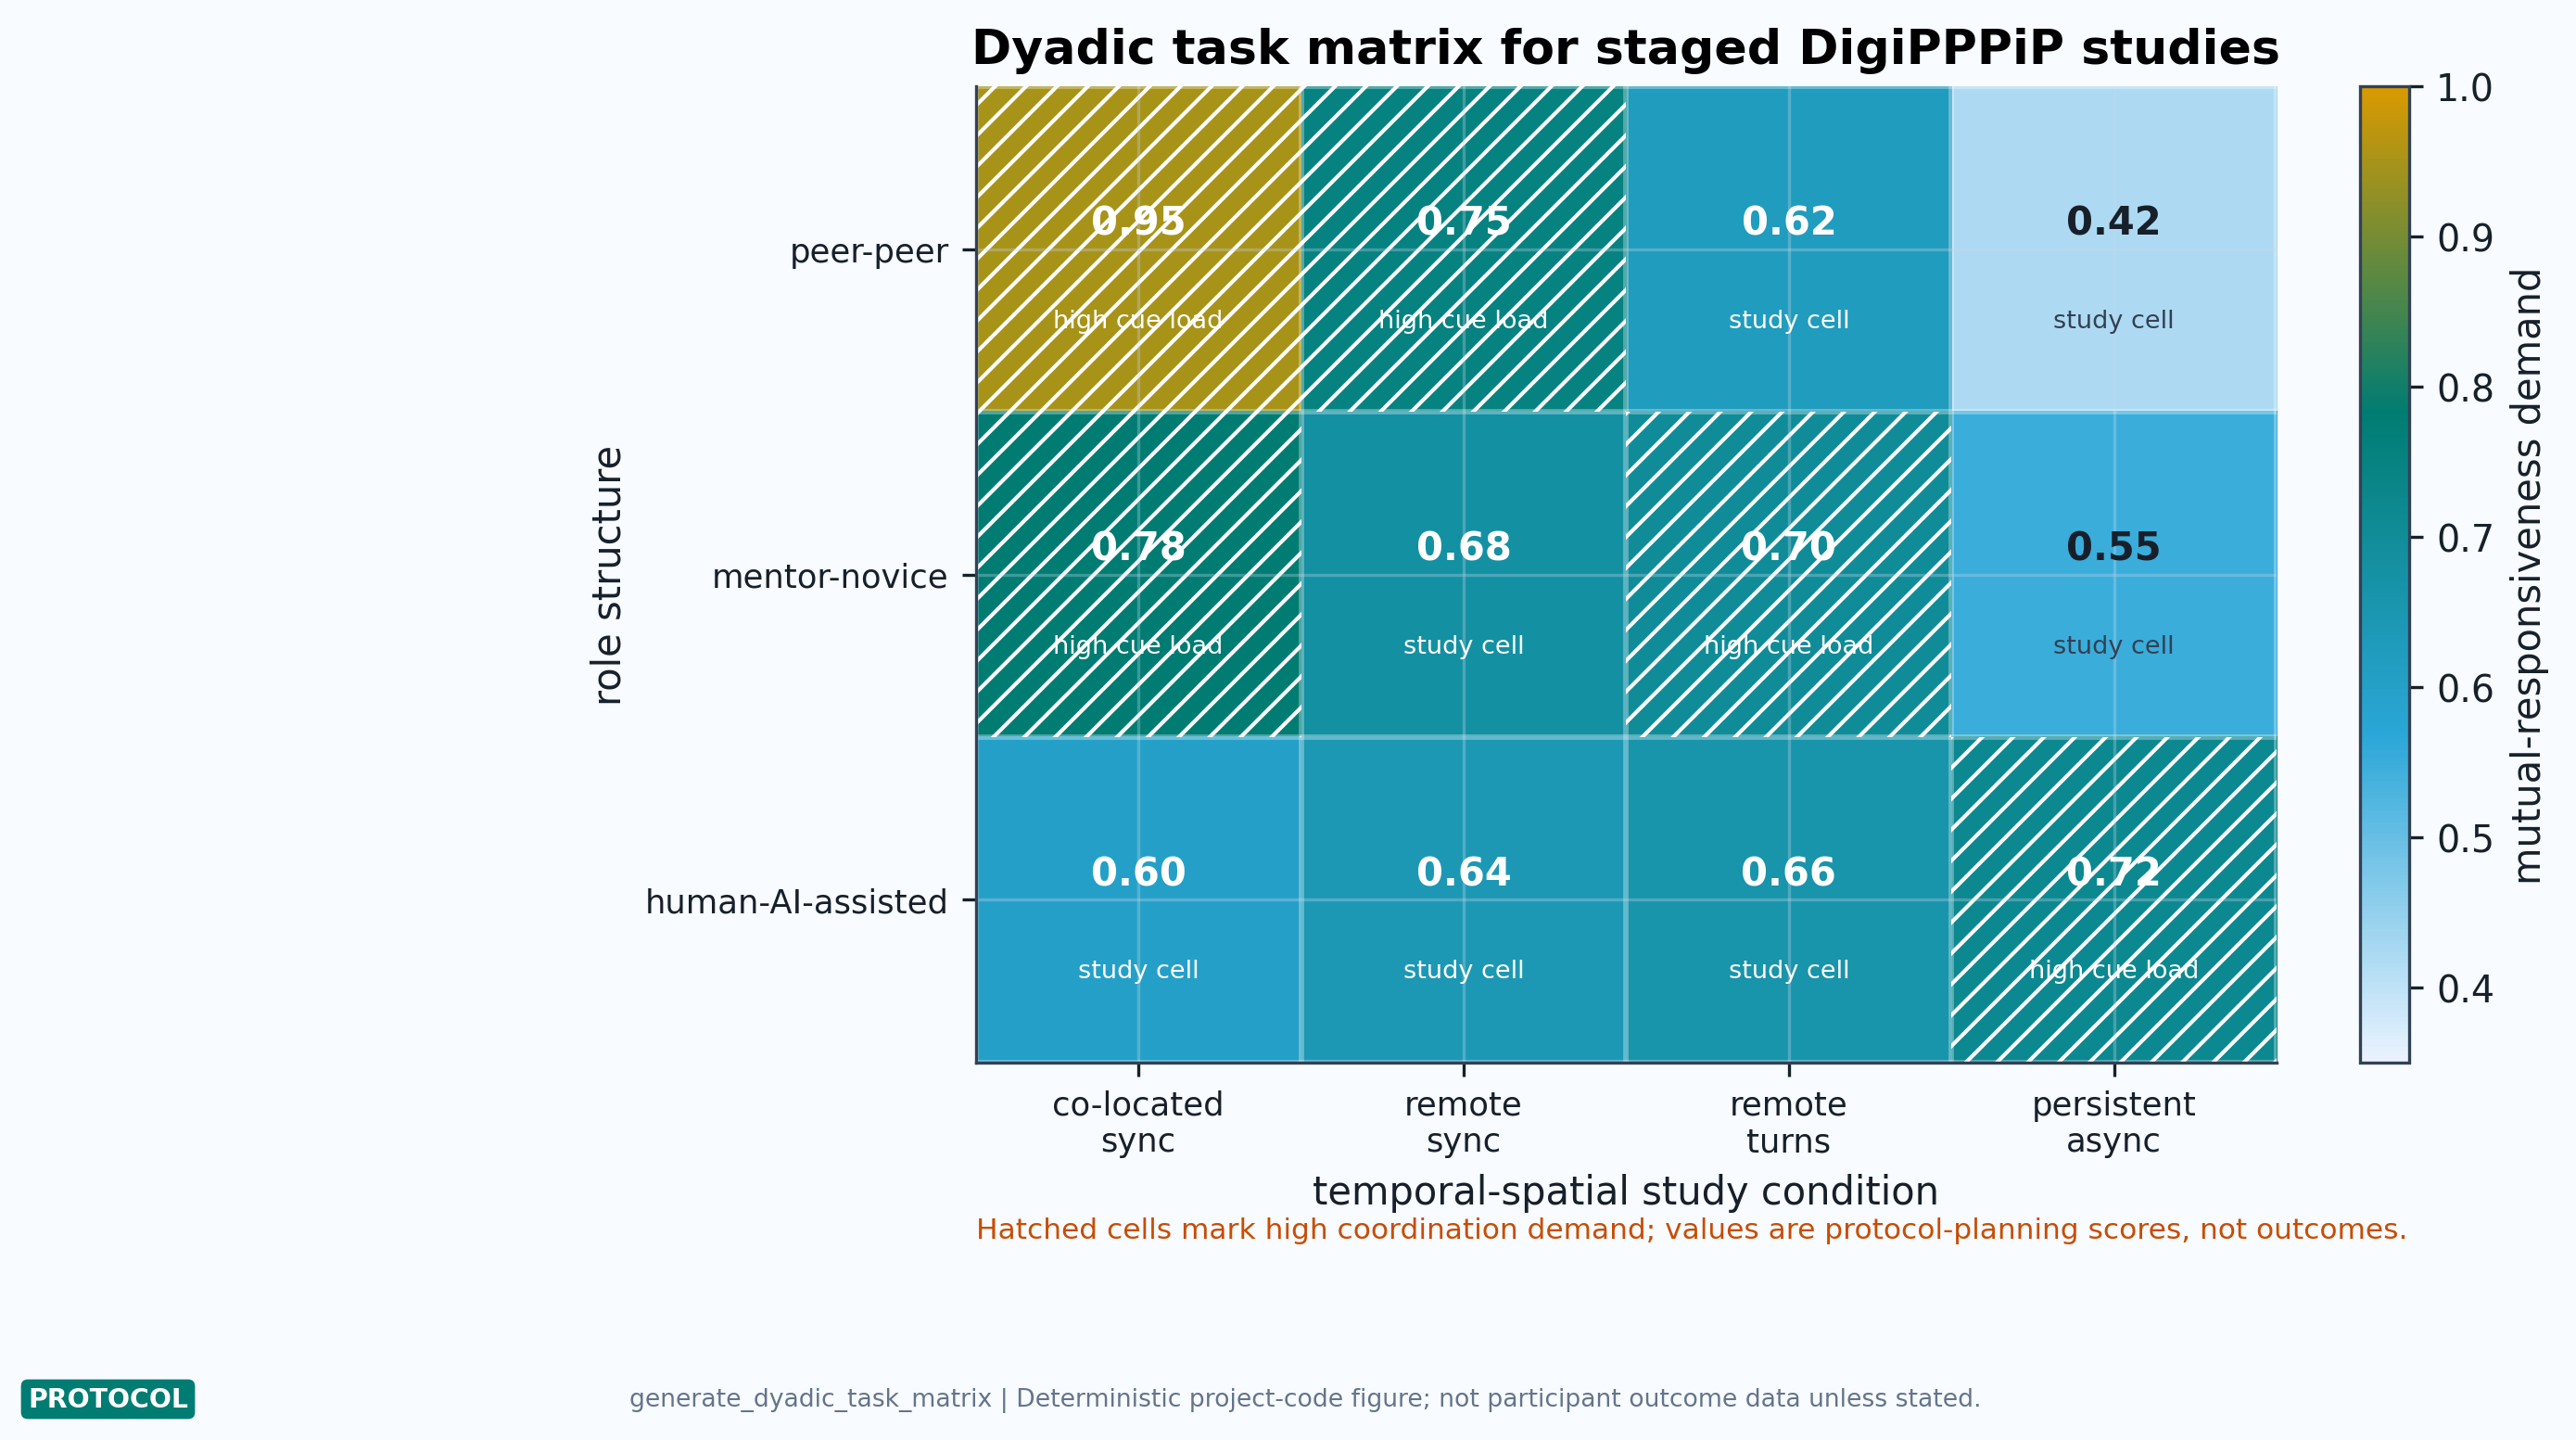
\includegraphics[width=0.9\linewidth,height=0.46\textheight,keepaspectratio,alt={Dyadic task matrix for staged DigiPPPiP studies. Values generated by generate\_dyadic\_task\_matrix() encode conceptual mutual-responsiveness demand across role structures and temporal-spatial conditions; read rows as partner-role arrangements, columns as session modes, numeric labels as planning scores, and patterned cells as high-coordination conditions. The matrix supports the temporal architecture's sampling argument rather than ranking modes as universally better. Empirical calibration would require observed timing logs, participant reports, and matched-condition comparisons.}]{../figures/dyadic_task_matrix.png}
\caption{Dyadic task matrix for staged DigiPPPiP studies. Values
generated by \protect\breaktt{generate\_dyadic\_task\_matrix()} encode
conceptual mutual-responsiveness demand across role structures and
temporal-spatial conditions; read rows as partner-role arrangements,
columns as session modes, numeric labels as planning scores, and
patterned cells as high-coordination conditions. The matrix supports the
temporal architecture's sampling argument rather than ranking modes as
universally better. Empirical calibration would require observed timing
logs, participant reports, and matched-condition
comparisons.}\label{fig:dyadic_task_matrix}
\end{figure}

\breakseq{[@fig:interaction\_timeline]} shows how the temporal distinction
becomes measurable. Strokes, utterances, repairs, and synchrony windows
occupy separate tracks so future studies can distinguish overlap,
alternation, latency, and delayed response without collapsing all of
them into a single session label.

\begin{figure}
\centering
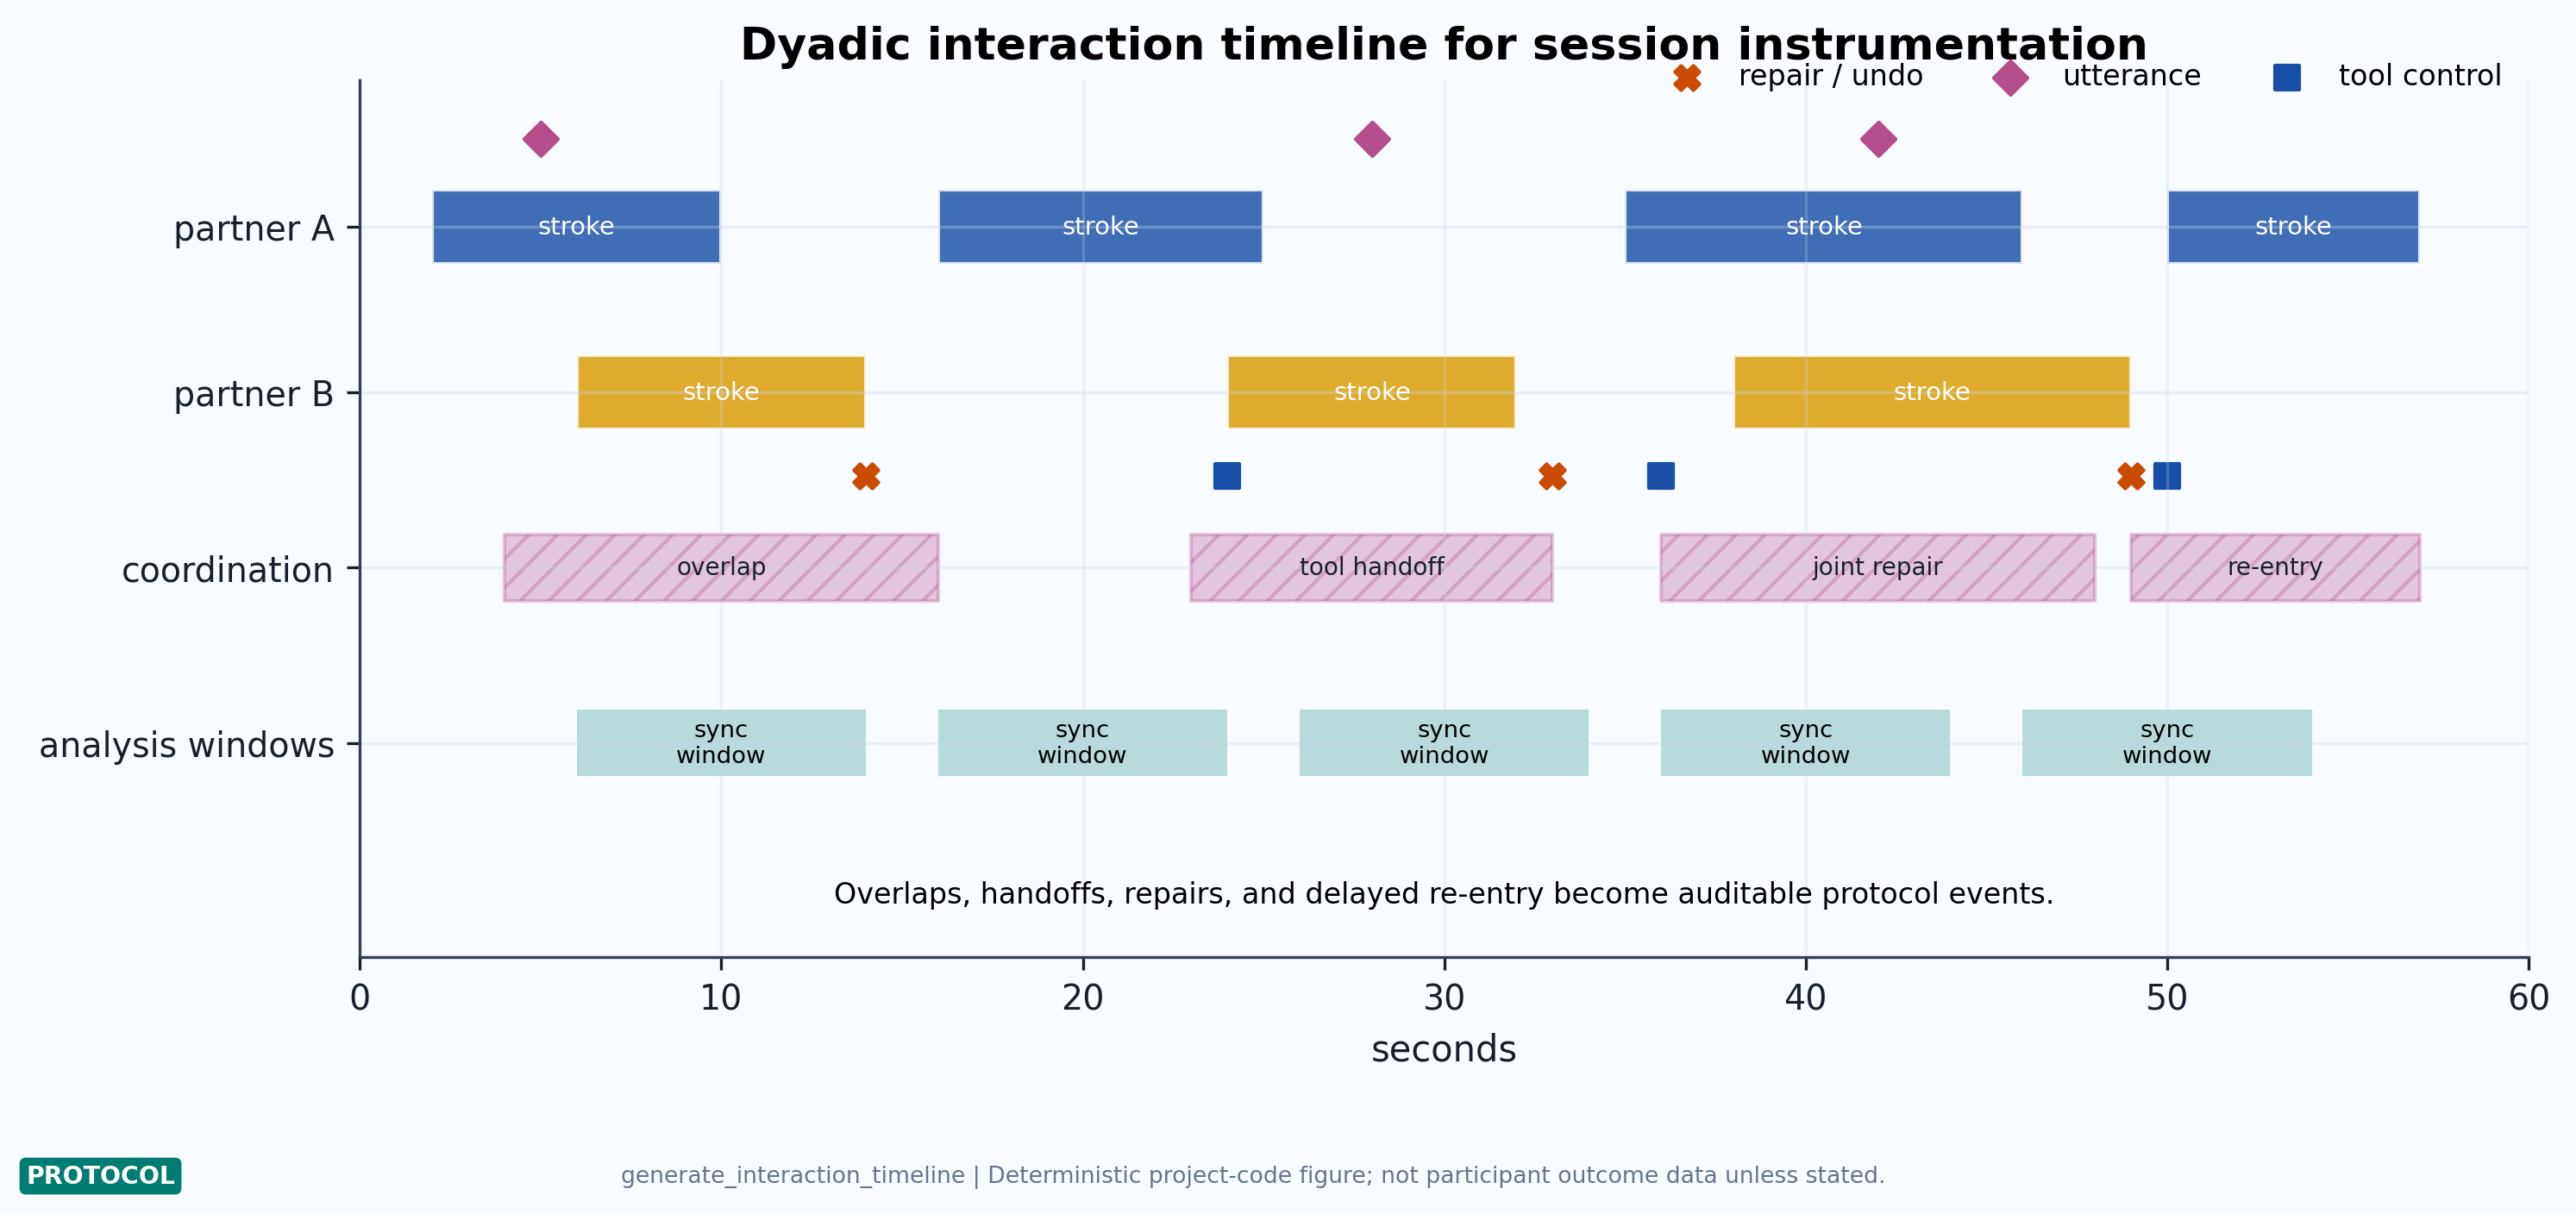
\includegraphics[width=0.9\linewidth,height=0.46\textheight,keepaspectratio,alt={Instrumented dyadic timeline linking partner actions, awareness cues, repair events, replay windows, and analysis windows. The figure is generated by generate\_interaction\_timeline(); read labelled bars as partner strokes, patterned spans as coordination windows, markers as utterances, tool-control changes, and repairs, and bottom bands as candidate analysis intervals. It supports the claim that temporal mode must be logged rather than asserted. The plot is a protocol schematic; participant data would replace the simulated intervals.}]{../figures/interaction_timeline.png}
\caption{Instrumented dyadic timeline linking partner actions, awareness
cues, repair events, replay windows, and analysis windows. The figure is
generated by \protect\breaktt{generate\_interaction\_timeline()}; read
labelled bars as partner strokes, patterned spans as coordination
windows, markers as utterances, tool-control changes, and repairs, and
bottom bands as candidate analysis intervals. It supports the claim that
temporal mode must be logged rather than asserted. The plot is a
protocol schematic; participant data would replace the simulated
intervals.}\label{fig:interaction_timeline}
\end{figure}

\breakseq{[@fig:parallel\_sequential\_patterns]} complements the timeline with
three canonical event patterns. The point is design clarity: parallel
marks, turn-taking marks, and long-delay marks invite different
hypotheses about attention, anticipation, and narrative continuity.

\begin{figure}
\centering
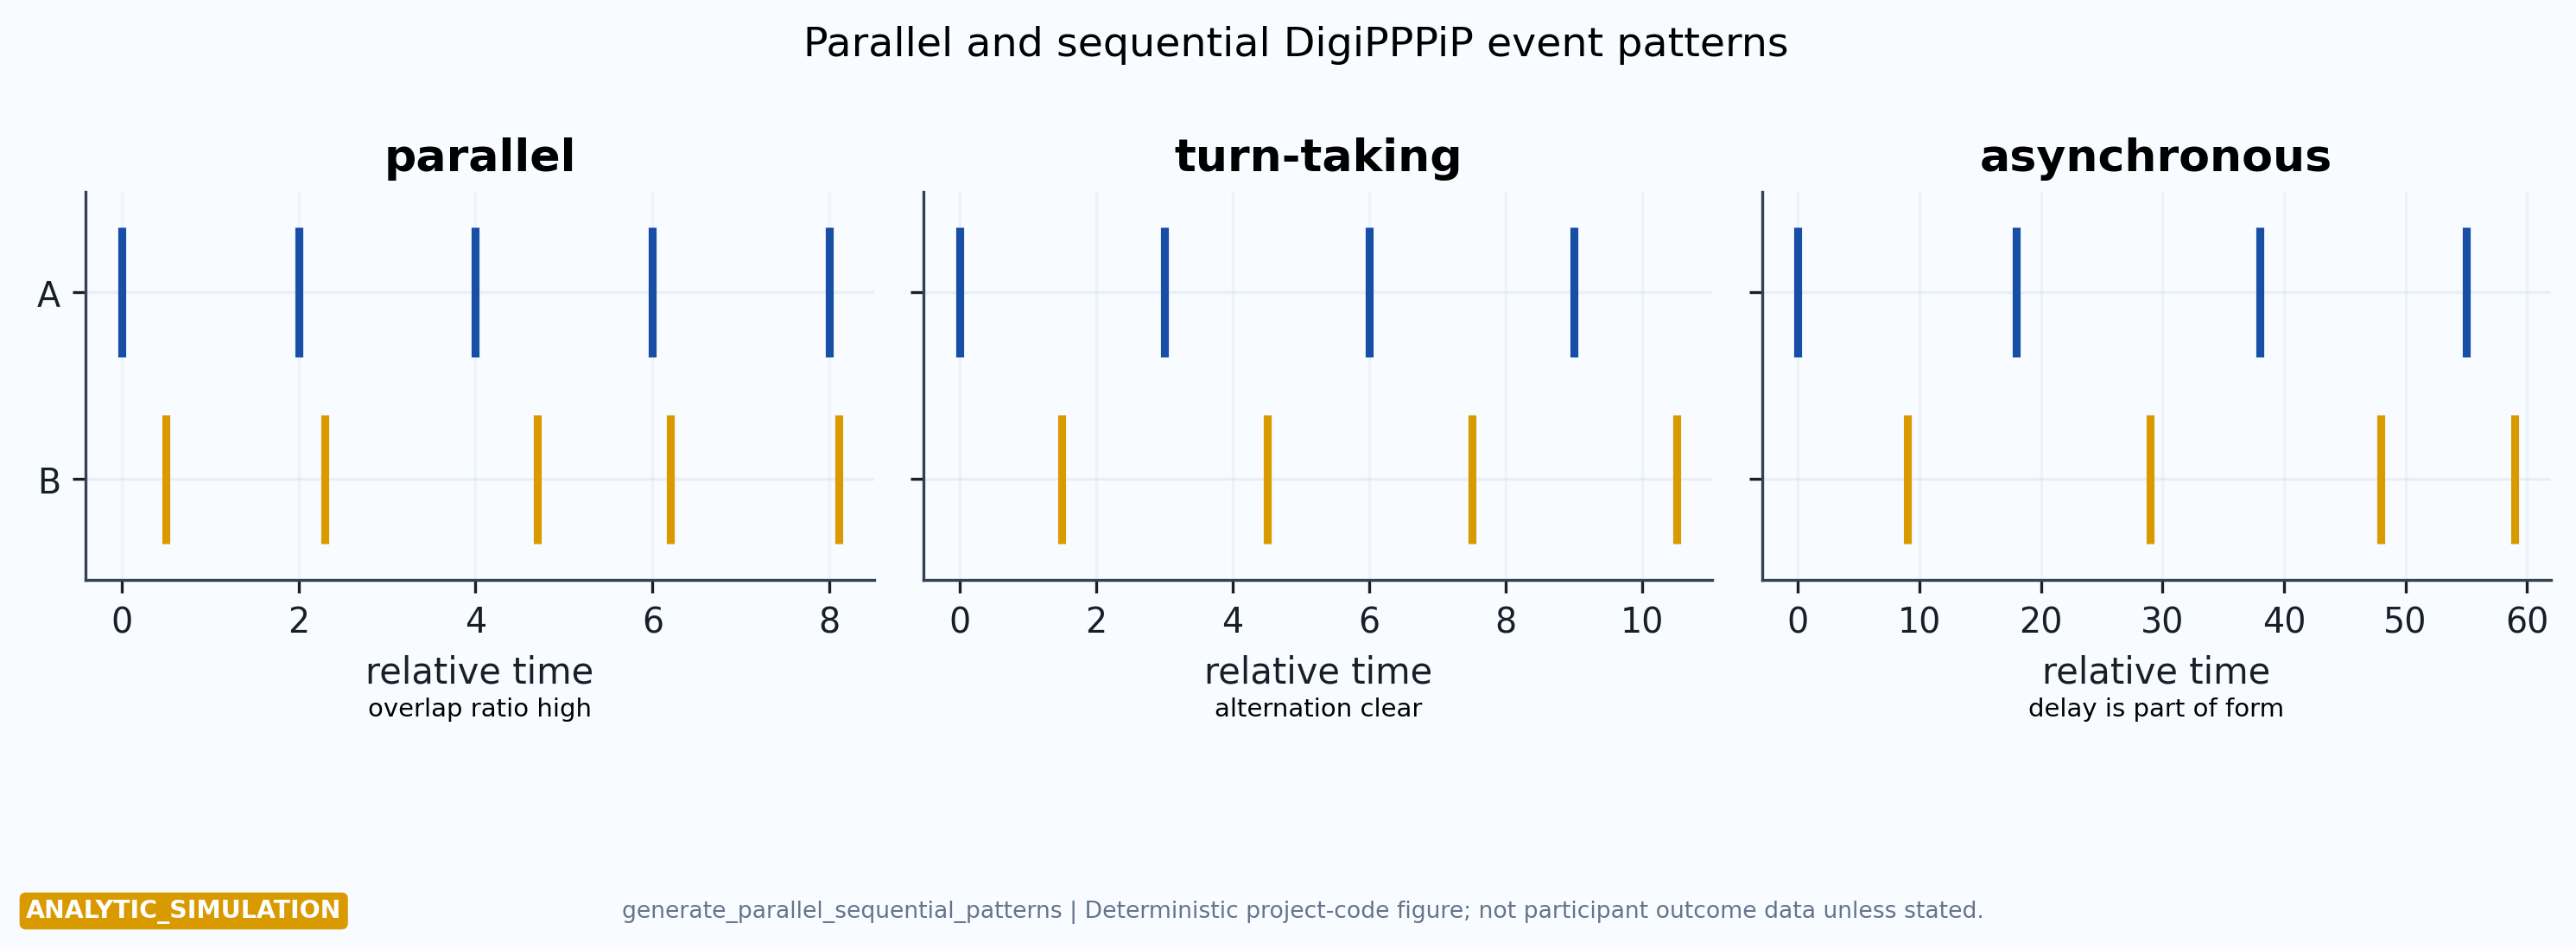
\includegraphics[width=0.9\linewidth,height=0.46\textheight,keepaspectratio,alt={Event-pattern comparison for parallel, turn-taking, and asynchronous DigiPPPiP sessions. The conceptual raster plots generated by generate\_parallel\_sequential\_patterns() use blue and orange event ticks to show overlap ratio, alternation, and long-delay response structure. The figure supports the temporal taxonomy by showing why synchrony, alternation, and persistence are different hypotheses. It is schematic; empirical use would require timestamped session logs.}]{../figures/parallel_sequential_patterns.png}
\caption{Event-pattern comparison for parallel, turn-taking, and
asynchronous DigiPPPiP sessions. The conceptual raster plots generated
by \protect\breaktt{generate\_parallel\_sequential\_patterns()} use blue
and orange event ticks to show overlap ratio, alternation, and
long-delay response structure. The figure supports the temporal taxonomy
by showing why synchrony, alternation, and persistence are different
hypotheses. It is schematic; empirical use would require timestamped
session logs.}\label{fig:parallel_sequential_patterns}
\end{figure}

\breakseq{[@fig:ibs\_phases]} gives a conceptual phase model for synchronous
sessions. It should not be read as empirical functional near-infrared
spectroscopy (fNIRS) output. Its role is to make explicit the hypothesis
that initiation, elaboration, convergence, and completion may differ in
inter-brain-synchrony profiles and should be tested directly.

\begin{figure}
\centering
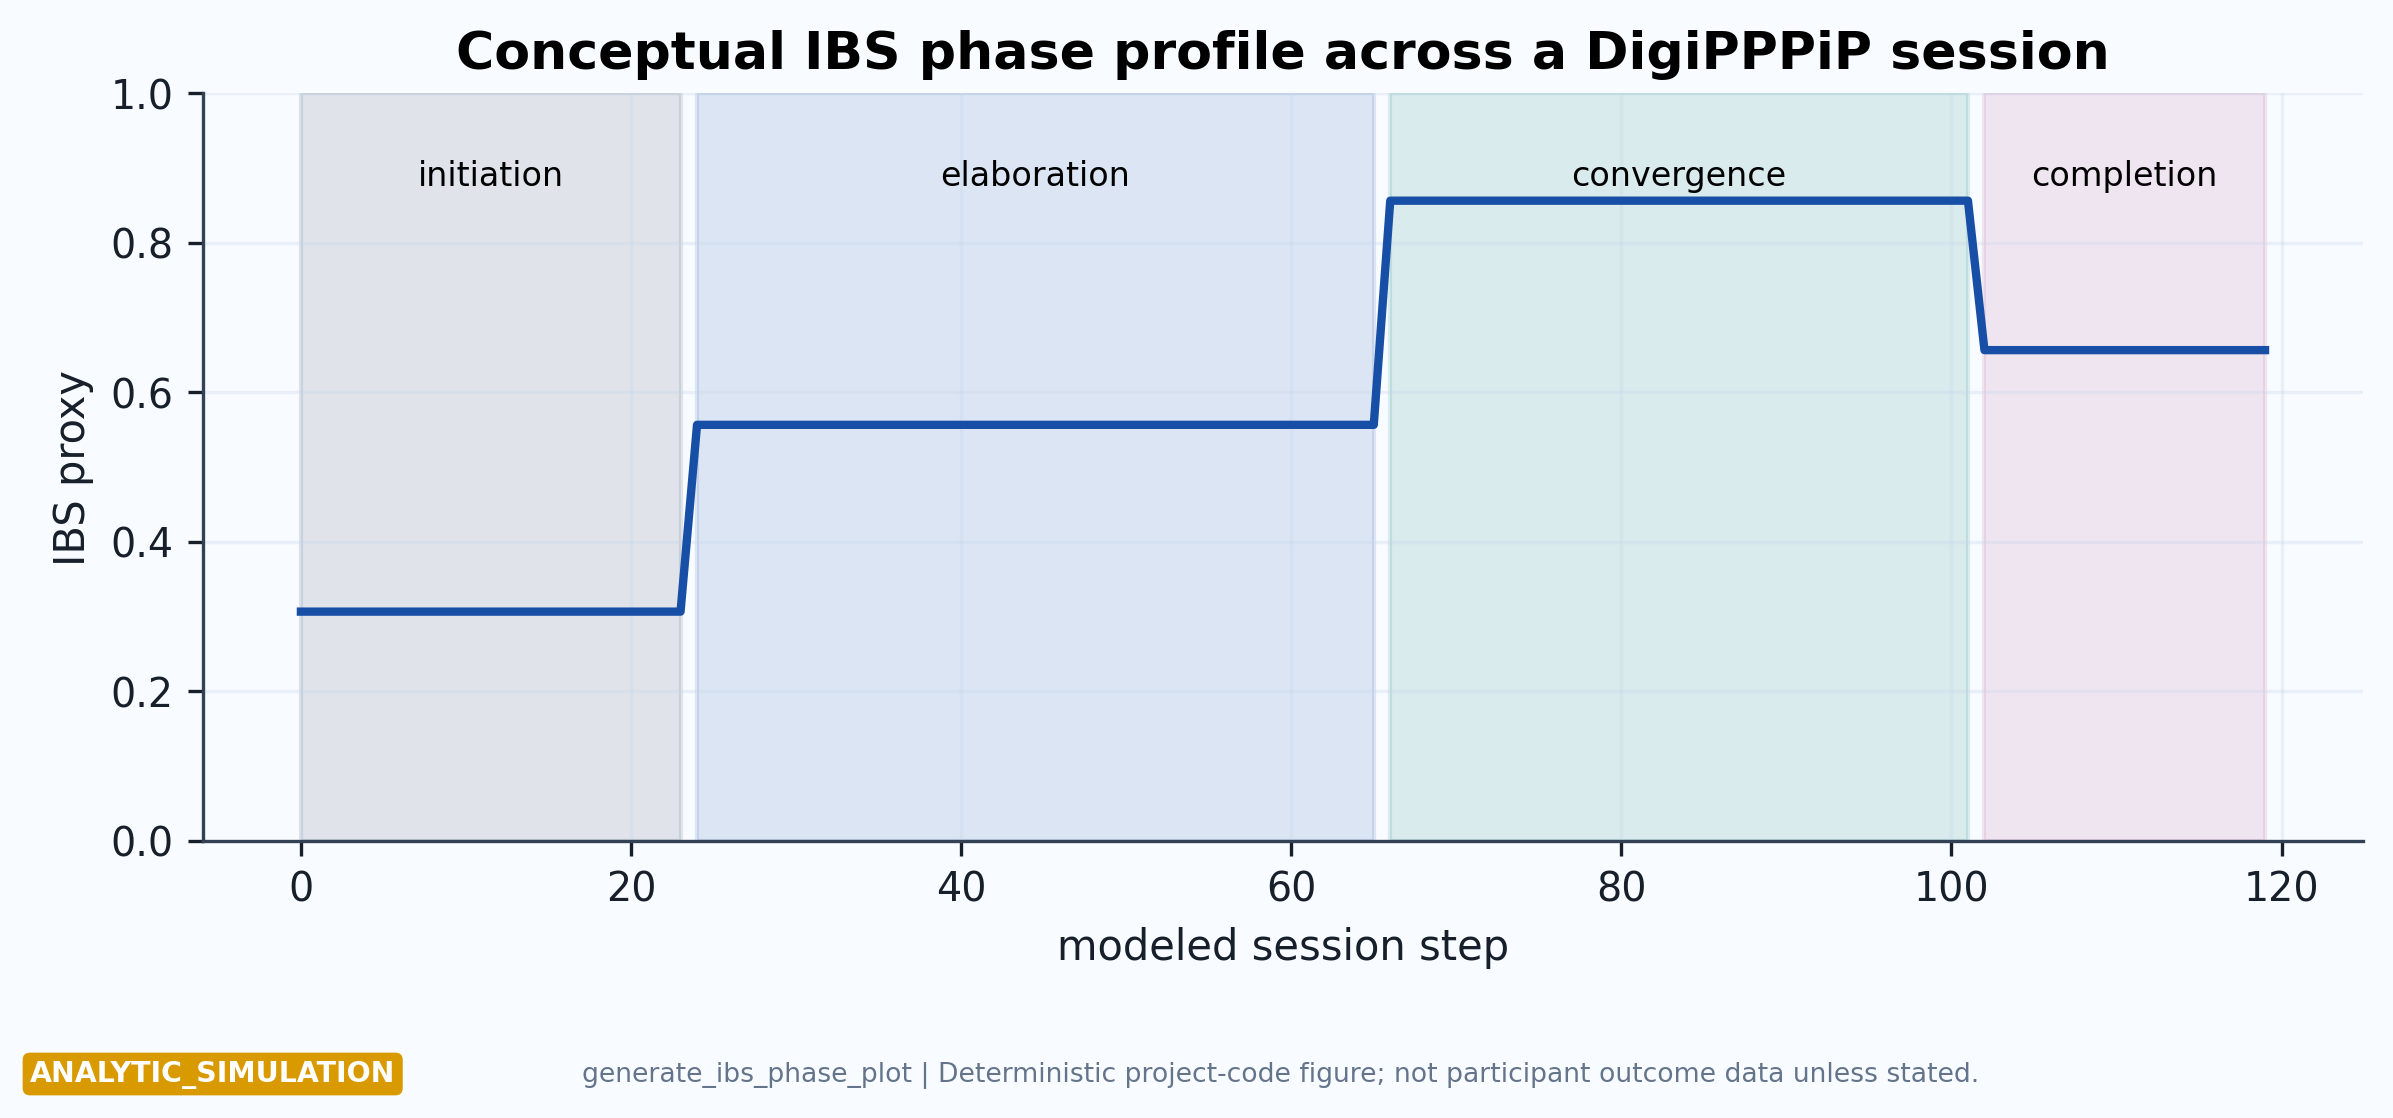
\includegraphics[width=0.9\linewidth,height=0.46\textheight,keepaspectratio,alt={Conceptual inter-brain-synchrony phase profile across initiation, elaboration, convergence, and completion. Values are generated by generate\_ibs\_phase\_plot() from src/hyperscanning.py; read the line as an illustrative synchrony proxy and shaded bands as session phases. The figure supports hypothesis formation for synchronous sessions, not neural evidence. Real fNIRS or electroencephalography (EEG) analyses would need artifact correction, controls, and preregistered phase definitions.}]{../figures/ibs_phases.png}
\caption{Conceptual inter-brain-synchrony phase profile across
initiation, elaboration, convergence, and completion. Values are
generated by \protect\breaktt{generate\_ibs\_phase\_plot()} from
\protect\breaktt{src/hyperscanning.py}; read the line as an illustrative
synchrony proxy and shaded bands as session phases. The figure supports
hypothesis formation for synchronous sessions, not neural evidence. Real
fNIRS or electroencephalography (EEG) analyses would need artifact
correction, controls, and preregistered phase
definitions.}\label{fig:ibs_phases}
\end{figure}
\end{frame}

\end{document}
